\documentclass[12pt,a4paper]{article}
\usepackage{amsmath}
\usepackage{amsfonts}
\usepackage{amssymb}
\usepackage{makeidx}
\usepackage{graphicx}
\usepackage{enumerate}
\usepackage{setspace}
\usepackage{longtable}
\usepackage{float}
\usepackage{hyperref}
\usepackage[framed,numbered,autolinebreaks,useliterate]{mcode}

\usepackage[left=2cm,right=2cm,top=1.75cm,bottom=1.75cm]{geometry}
\author{N Sowmya Manojna}

\usepackage{fontspec}
\setmainfont{Cambria}

\usepackage{caption}
\DeclareCaptionLabelSeparator{pipe}{ $|$ }% or $\vert$
\captionsetup{font=small, labelfont={bf, color=blue}}

\newcommand{\spa}{\vspace{1.5em}}
\newcommand{\noi}{\noindent}
\def\dul#1{\underline{\underline{#1}}}


\begin{document}
\begin{titlepage}
	\begin{center}
		\vspace{3em}
		\large {BT6270 Computational Neuroscience}
		\vspace{10em}

		\rule{0.9\linewidth}{0.5mm} \\[0.4cm]
	    \large{\bfseries{Computational Neuroscience Assignment 2}} \\
	    \rule{0.9\linewidth}{0.5mm} \\[3 em]

	    N Sowmya Manojna | BE17B007\\
		Department of Biotechnology,\\
		Indian Institute of Technology, Madras\\

		\vspace{5em}
		
\includegraphics[scale = 0.09]{images/iitmlogo.png}

	\end{center}
\end{titlepage}

\noi
The FitzHugh Nagumo model is a relaxation oscillator \cite{wiki} that is obtained from simplification of the detailed Hodgkin-Huxley model. This simplification is obtained by condensing the ion channel activations into a $w$ variable.\\

The two variable FitzHugh-Nagumo model can be simulated using the following equations:
$$
\frac{dv}{dt} = v(a-v)(v-1) - w + I_{ext}\\
$$
$$
\frac{dw}{dt} = bv-rw
$$

The parameters used in the first three Cases are are:
$$
a = 0.5,  b = 0.1, r = 0.1
$$

\section{Case 1: $I_{ext} = 0$}
\subsection{Phase Plot}
	\begin{figure}[H]
	\centering
	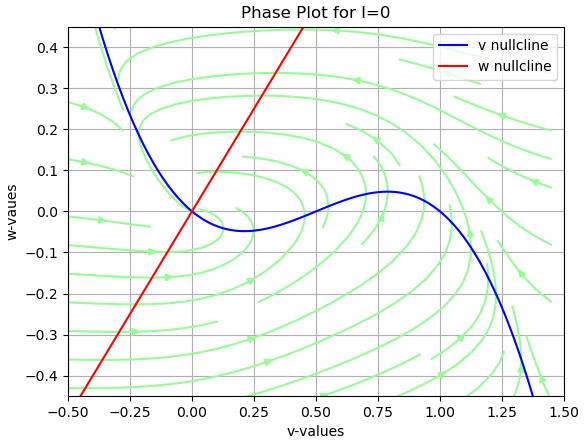
\includegraphics[scale=0.6]{images/Figure_1.png}
	\caption{Phase Plot of the system when $I_{ext} =  0$. The stationary point obtained is a stable point.}
	\end{figure}

	Analyzing the trajectories by using initial points - $[0, 0.4, 0.6, 1], w=0$, we can see that even for perturbations in the initial start point, we approach the equilibrium point at $[0,0]$. Hence, the point $[0,0]$ is a stable fixed point.

	\begin{figure}[H]
	\centering
	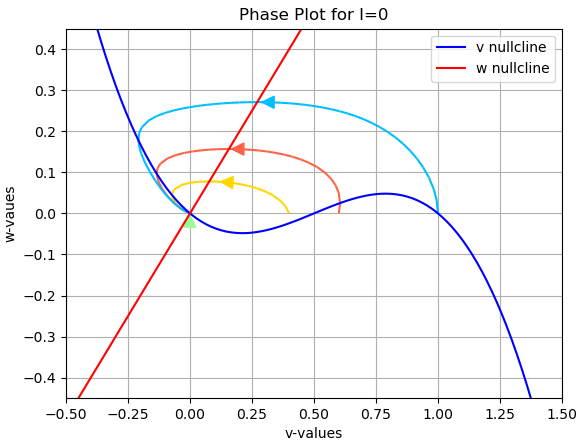
\includegraphics[scale=0.6]{images/Figure_2.png}
	\caption{Stability analysis of the equilibrium point. The model approaches the equilibrium point irrespective of the initial conditions. Hence, the equilibrium point is a stable fixed point.}
	\end{figure}

\subsection{$V(t), W(t)$ across $t$, Trajectories}
	For an $I_{ext}$ value of 0, no action potentials are observed.	
	\begin{figure}[H]
	\centering
	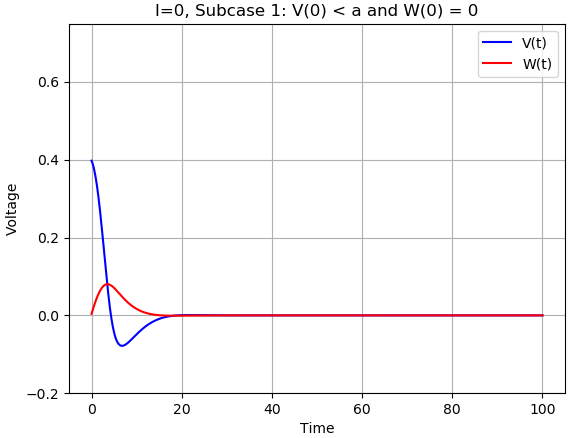
\includegraphics[scale=0.6]{images/Figure_3.png}
	\caption{$V(t), W(t)$ across $t$, when $V(0)<a$. With sub-threshold pulse injections, no action potentials are observed.}
	\end{figure}

	\begin{figure}[H]
	\centering
	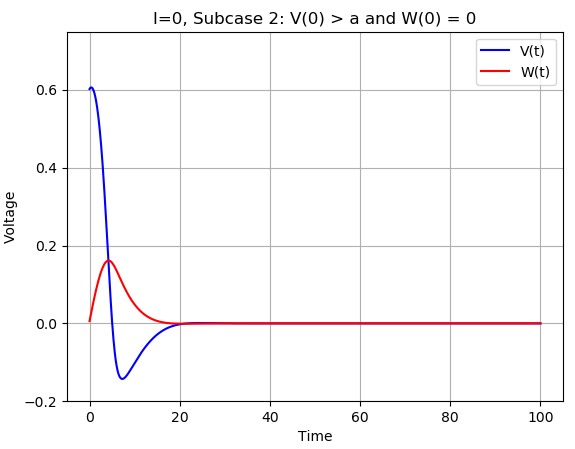
\includegraphics[scale=0.6]{images/Figure_4.png}
	\caption{$V(t), W(t)$ across $t$, when $V(0)>a$. With sub-threshold pulse injections, no action potentials are observed.}
	\end{figure}

\section{Case 2: $I_{ext}=0.6$}
\subsection{Phase Plot}
	\begin{figure}[H]
	\centering
	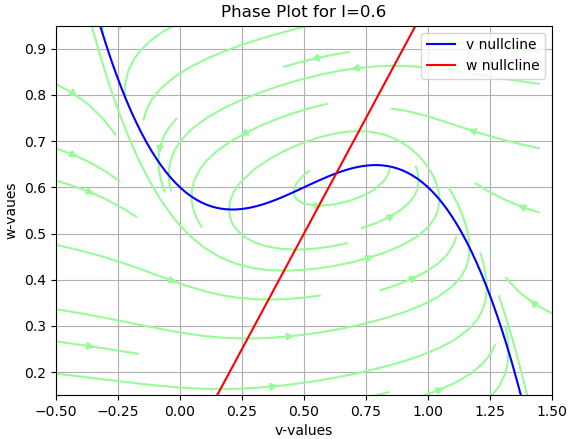
\includegraphics[scale=0.6]{images/Figure_5.png}
	\caption{Phase Plot of the system when $I_{ext} =  0.6$. This stationary point is found to be a unstable point.}
	\end{figure}

	The trajectories were analyzed by using initial points - $[0, 0.4, 0.6, 1], w=0$. We can see that at the point of intersection of the nullclines, there are circulating fields around the unstable stationary point. Additionally we also see limit cycle enclosing the stationary point.

	\begin{figure}[H]
	\centering
	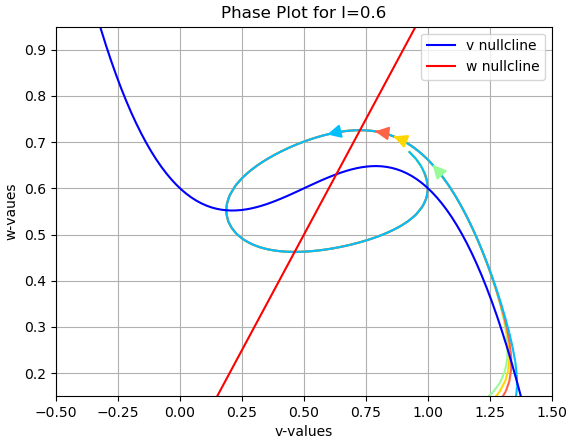
\includegraphics[scale=0.6]{images/Figure_6.png}
	\caption{Stability analysis of the stationary point. The stationary point is found to be unstable and limit cycle behavior is also observed.}
	\end{figure}

\subsection{$V(t), W(t)$ across $t$, Trajectories}
	For $I_{ext}=0.6$, oscillatory membrane potential is seen in the limit cycle region.
	\begin{figure}[H]
	\centering
	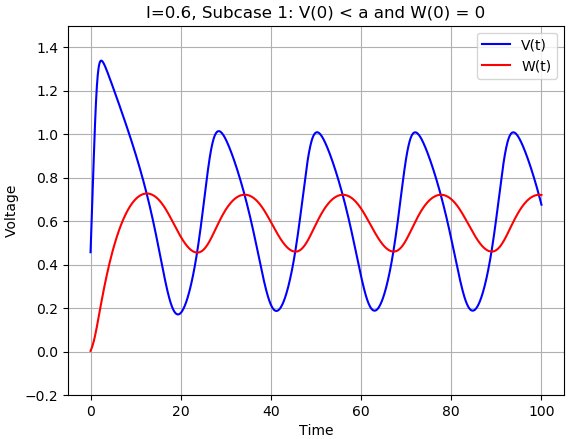
\includegraphics[scale=0.6]{images/Figure_7.png}
	\caption{$V(t), W(t)$ across $t$, when $V(0)<a$. Sustained oscillations are observed.}
	\end{figure}

	\begin{figure}[H]
	\centering
	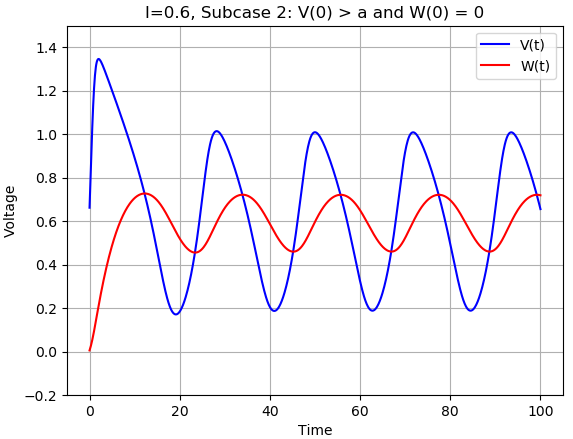
\includegraphics[scale=0.6]{images/Figure_8.png}
	\caption{$V(t), W(t)$ across $t$, when $V(0)>a$. Sustained oscillations are observed.}
	\end{figure}

\section{Case 3: $I_{ext}=1$}
\subsection{Phase Plot}
	\begin{figure}[H]
	\centering
	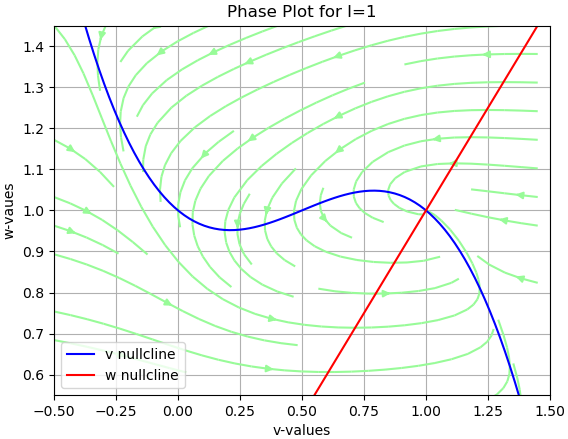
\includegraphics[scale=0.6]{images/Figure_9.png}
	\caption{Phase Plot of the system when $I_{ext} =  1$. This stationary point is found to be a stable point.}
	\end{figure}

	The trajectories were analyzed by using initial points - $[0, 0.4, 0.6, 1], w=0.6$ and $[0, 0.4, 0.6, 1], w=1.4$. We can see that even for large perturbations in the initial start point, we approach the equilibrium point at $[1,1]$. Hence, the point $[1,1]$ is a stable fixed point.

	\begin{figure}[H]
	\centering
	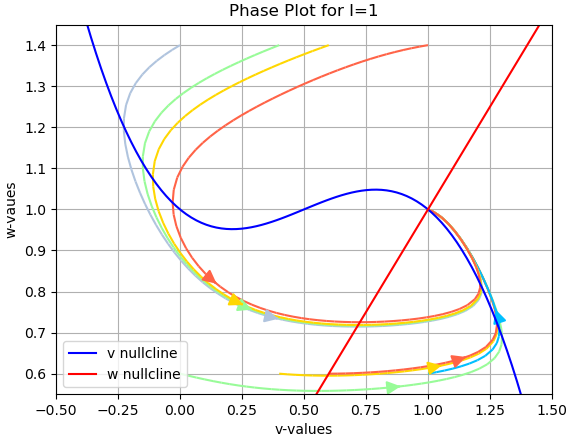
\includegraphics[scale=0.6]{images/Figure_10.png}
	\caption{Stability analysis of the stationary point. This stationary point is found to be a stable point.}
	\end{figure}

\subsection{$V(t), W(t)$ across $t$, Trajectories}
	For $I_{ext}=1$, depolarization is observed in the membrane potential. The voltage initially rises and then stays at a high value.
	\begin{figure}[H]
	\centering
	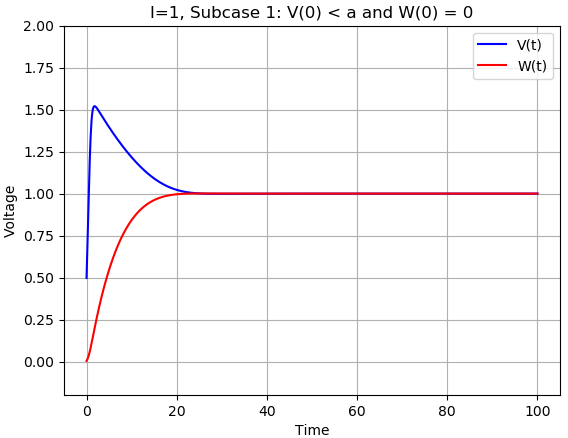
\includegraphics[scale=0.6]{images/Figure_11.png}
	\caption{$V(t), W(t)$ across $t$, when $V(0)<a$. With sub-threshold pulse injections, depolarization in the action potential can be observed.}
	\end{figure}

	\begin{figure}[H]
	\centering
	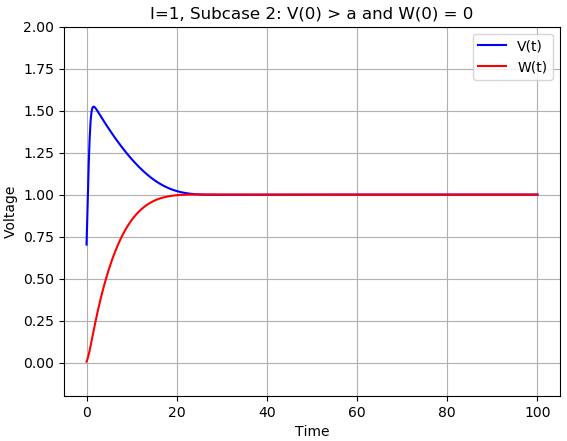
\includegraphics[scale=0.6]{images/Figure_12.png}
	\caption{$V(t), W(t)$ across $t$, when $V(0)>a$. With sub-threshold pulse injections, depolarization in the action potential can be observed.}
	\end{figure}

\section{Case 4: $I_{ext}=0.02$}
The parameter values used to simulate this case are: $b=0.01, r=0.8$. Hence, $b/r = 0.0125$.
\subsection{Phase Plot}
	\begin{figure}[H]
	\centering
	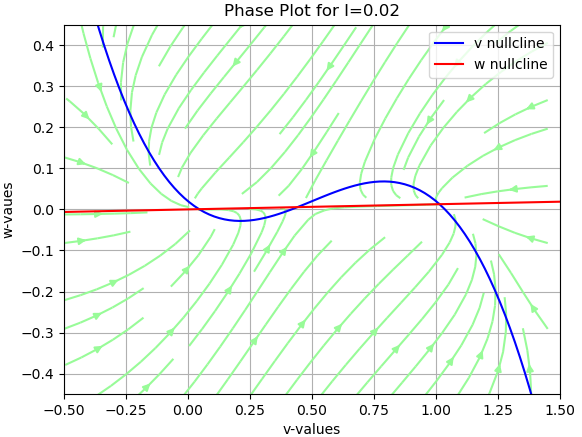
\includegraphics[scale=0.6]{images/Figure_13.png}
	\caption{Phase Plot of the system when $I_{ext} =  0.02$. The stationary points P1, P2 and P3 in that order are stable, saddle and stable points respectively.}
	\end{figure}

	The trajectories were analyzed by using initial points - $[0, 0.4, 0.6, 1], w=0.6$ and $[0, 0.4, 0.6, 1], w=1.4$. The stationary points are P1, P2 and P3, in that order. In case of P1 and P3 - small and intermediate perturbations lead back to P1 and P3 respectively. Hence P1 is a stable point. In case of P2, small perturbations along one axis leads to large change in final point. Hence, P2 is a saddle node. 

	\begin{figure}[H]
	\centering
	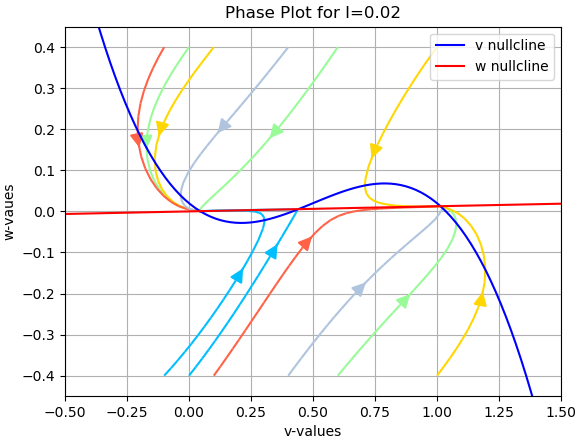
\includegraphics[scale=0.6]{images/Figure_14.png}
	\caption{Stability analysis of the stationary point. The stationary point is found to be unstable and limit cycle behavior is also observed.}
	\end{figure}

\subsection{$V(t), W(t)$ across $t$, Trajectories}
	For $I_{ext}=0.02, r=0.8, b=0.01$, bi-stability is observed.
	\begin{figure}[H]
	\centering
	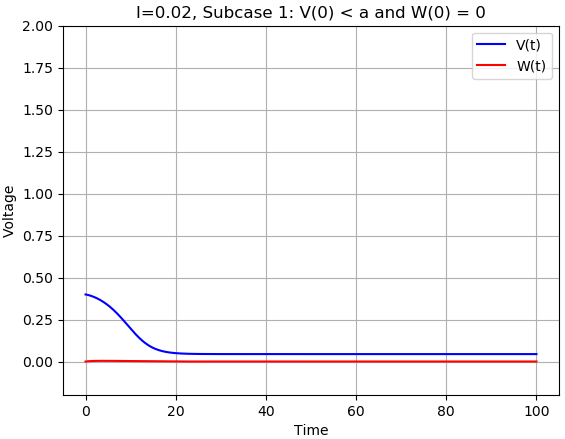
\includegraphics[scale=0.6]{images/Figure_15.png}
	\caption{$V(t), W(t)$ across $t$, when $V(0)<a$. The neuron exists in a tonically down state.}
	\end{figure}

	\begin{figure}[H]
	\centering
	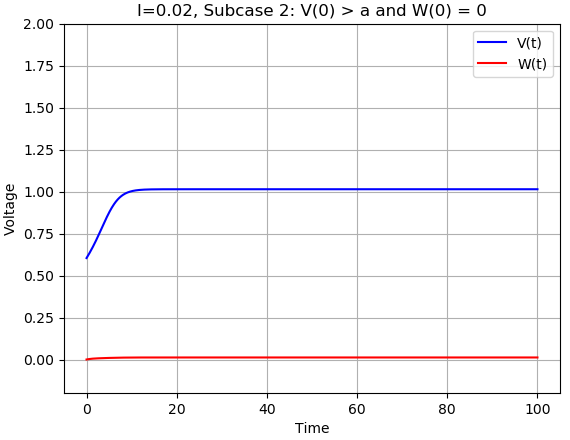
\includegraphics[scale=0.6]{images/Figure_16.png}
	\caption{$V(t), W(t)$ across $t$, when $V(0)>a$. The neuron exists in a tonically up state.}
	\end{figure}



\break
\bibliographystyle{ieeetr}
\bibliography{references.bib}
\end{document}
